\documentclass{classes/base}

\title{Manuale utente}
\versione{ inserire }
\author{\angela }
\verificatore{ inserire}
\approvatore{ inserire }
\uso{Esterno}

\begin{document}
	\maketitle
	\newpage
	\section*{Registro delle modifiche}
{

\newlength{\freewidth}
\setlength{\freewidth}{\dimexpr\textwidth-10\tabcolsep}
\renewcommand{\arraystretch}{1.5}
\centering
\setlength{\aboverulesep}{0pt}
\setlength{\belowrulesep}{0pt}
\rowcolors{2}{Arancione!10}{white}
\begin{longtable}{C{.13\freewidth} C{.15\freewidth} C{.26\freewidth} C{.18\freewidth} C{.282379\freewidth}}
	\toprule
\rowcolor{Arancione}
\textcolor{white}{\textbf{Versione}}&
\textcolor{white}{\textbf{Data}}&
\textcolor{white}{\textbf{Nominativo}}&
\textcolor{white}{\textbf{Ruolo}}&
\textcolor{white}{\textbf{Descrizione}}\\	
\toprule
\endhead

0.0.3 & 01-09-2022 & \angela{} & Analista & Inserite le informazioni mancati (Verficatore: )\\	
0.0.2 & 22-08-2022 & \angela{} & Analista & Inserite le sezioni dalla 4 alla 10 (verificatore: )\\	
0.0.1 & 22-08-2022 & \giulio{} & Analista & Stesura Intro (Verficatore: \angela)\\
0.0.0 & 20-08-2022 & \angela{} & Analista & Creazione documento\\	
\bottomrule
\end{longtable}
}

	\newpage
	\tableofcontents
	\newpage
	\listoffigures

	\newpage
    \section{Introduzione}

\subsection{Scopo del documento}
Lo scopo del seguente documento è il voler illustrare
le relative funzionalità che la WebApp BunnyFood vuole offrire.
Per ogni funzionalità viene associata una dettagliata spiegazione di essa e
il suo relativo funzionamento.

\subsection{Scopo del prodotto}
Lo scopo principale della WebApp BunnyFood e dell'azienda Zero12 è quello di poter fornire all'utente delle guide
relative a delle località (di ristorazione, o semplici luoghi di interesse) basandosi sui contenuti creati e condivisi dagli utenti
della principale piattaforma social (Instagram). 
La piattaforma BunnyFood, inoltre è capace di effettuare una classfica delle guide generata tramite le impressioni e le reazioni degli utenti 
che utlizzano la piattaforma social.

\subsection{Glossario}
E' stato redatto il documento "Glossario v2.0.0" con lo scopo di illustrare nuove terminologie utlizzate.
Il documento contiene spiegazioni dei termini più importanti che sono stati usati nei documenti, e tali termini
vengono segnalati con l'apice G.

\subsection{Riferimenti}
\begin{itemize}
	\item
	{\textbf{Regolamento progetto didattico}}\\\url{https://www.math.unipd.it/~tullio/IS-1/2021/Dispense/PD2.pdf}

\end{itemize}


	\newpage
    \section{Requisiti di sistema}
Per poter accedere alle funzionalità della WebApp\G{} è necessario soddisfare i seguenti requisiti:

\subsection{Prerequisiti}
L'unico prerequisito necessario ed obbligatorio per utilizzare la WebApp\G{} \platform{} è l'aver attivato \textbf{JavaScript}\G{} sul proprio browser.

\subsection{Requisiti software}
La WebApp\G{} \platform{} richiede le seguenti caratteristiche minime software per il suo corretto funzionamento:\\

\textbf{Sistema operativo}
\begin{itemize}
    \item Windows
    \item Ubuntu 
    \item Mac Os X
    \item iOS
    \item Android
\end{itemize}

\textbf{Browser}
\begin{itemize}
    \item Google Chrome (da versione 104.0.5112.102)
    \item Mozilla Firefox (da versione 104.0)
    \item Safari (da versione 15.5)
    \item Microsoft Edge (da versione 104.0.1293.47)
\end{itemize}

\subsection{Segnalazione problematiche}
Nel caso ci si imbatta in problematiche riguardanti il funzionamento di \platform, è possibile
effettuare una segnalazione scrivendo una mail al seguente indirizzo:\\


\begin{center}
email: \textbf{\href{mailto:bugsbunnyteam@protonmail.com}{bugsbunnyteam@protonmail.com} }
\end{center}


	\newpage
    \section{Accesso alla WebApp} {
    Per accedere, e quindi visualizzare e utilizzare le funzionalità della WebApp, si può seguire il seguire indirizzo web:
    
    \begin{center}
        \textbf{Link}
    \end{center}



    Dal momento della visualizzazione della WebApp, è possibile sfruttare le sue funzionalità, le quali:
    \begin{itemize}
        \item Registrazione (se l'utente è sprovvisto di account)
        \item Login 
        \item Recupero password (se l'utente ha scordato la sua password personale)
        \item Visualizzazione del proprio account \begin{itemize}
            \item Modifica password,
            \item Modifica tipologia di vista predefinita per le guide (lista o mappa),
            \item Visualizzare la lista dei propri seguaci (con possibilità di rimozione di un seguace),
        \end{itemize}
        \item Visualizzazione della Home (l'utente ha la possibilità di scegliere il tipo di visualizzazione, lista o mappa)
        \item Logout
    \end{itemize}

}


    \newpage
    \section{Registrazione} {

Per accedere ai servizi, gratuiti e accessibili da chiunque, della piattaforma \platform  è necessario eseguire la registrazione tramite il seguente link:
\begin{center}
    \textbf{mettere il link} 
\end{center} 
La registrazione permette di creare un account personale al quale verrà illustrata una guida sottoforma di mappa o lista con i luoghi più apprezzati dai clienti e 
inoltre è possibile iniziare a seguire dei nuovi profili Instagram. \aCapo
Per effettuare la registrazione sulla piattaforma \platform è necessario procedere come spiegato seguentemente: \aCapo 
Premere il bottone con il testo "\textbf{Registrazione}" (non so ancora dove sarà collocato con Cognito).
Allegare foto! \aCapo
Dopo aver cliccato sul bottone, si viene reindirizzati in una pagina nuova, contente il seguente form, nel quale verranno inseriti i dati necessari per completare 
correttamente tale passaggio. \aCapo
I dati richiesti sono i seguenti:
\begin{itemize}
    \item Nomeutente 
    \item Indirizzo email
    \item Password
    \item Conferma password
\end{itemize}
Nel campo "Indirizzo email" verrà effettuato un controllo per assicurarsi che il formato inserito sia corretto. (anche gli altri campi avranno dei controlli? boh) \aCapo
Quando tutti i campi sono stati compilati bisogna cliccare il pulsante con il testo "Registrati". \aCapo

Non so ancora esattamente cosa succederà dopo. 

\subsection{Inserimento dati errati} {
Se l'utente lascia anche solo un campo vuoto dei 4 del form di registrazione, comparirà un messaggio d'errore (come mostrato in figura) e 
la registrazione non sarà avvenuta. 

FOTO 


}

}


	\newpage
	\section{Login} {
    Per effutare il login, è possibile eseguirlo accedendo tramite il link segunte: 
    \begin{center}
        \textbf{mettere il link}
    \end{center}
    \subsection{Login manuale} {
        L'utente per accedere alla piattaforma deve cliccare il pulsante "\textbf{Login}", succesivamente verrà indirizzato ad una nuova pagina, 
        la quale contine il form da compilare. I campi da inserire sono: 
        \begin{itemize}
            \item Nomeutente
            \item Password
            \item Memorizza sessione
        \end{itemize}
        I dati da inserire sono esattamente quelli con cui era avvenuta la registrazione. \aCapo
        Per accedere alla piattoforma è necessario premere il bottone "\textbf{Login}". \aCapo
        Se andrà a buon fine, l'utente una volta entrato nella piattaforma potrà visitare la propria home, accedere all'area personale ed infine usufruire dei servizi disponibili da \platform.
        \subsection{Inserimento delle credenziali errate} {
            Se uno o entrambi i campi del modulo di Login non vengono completati, il sistema darà errore come si vede dalla figura. Infatti per accedere è necessario completare i campi, e assicurarsi
            che essi contengano le credenziali scritte corretamente, altriemnti verrà segnalato un errore di quest'altro tipo: 
        }   
    }

    \subsection{Login automatico} {
        Se l'utente durante una fase di login precedente, aveva spuntato la casella per memorizzare la sessione di login, una volta premuto il 
        bottone di "\textbf{Login}" verrà reindirizzato direttamnete alla pagina home della piattaforma, perchè non sarà necessario inserire nuovamente le proprie credenziali.
    
    }
    
    \subsection{Logout} {
        Quando un utente sta navigando all'interno di \platform, per uscire da essa deve eseguire il logout. Per farlo deve cliccare sul bottone "\textbf{Account}", il quale lo reindirizzerà ad una nuova pagina,
        nella quale saranno presente le informazioni personali e il bottone "\textbf{Logout}" che gli permterrà di uscire da \platform. 
          
    }




}


	\newpage
	\section{Recupero password} {
    Nel caso in cui l'utente, al momento del login, avesse dimenticato la propria password per accedere alla piattaforma 
    \platform può recuperarla premendo il link "\textbf{Forgot my password}". 
    \begin{figure}[H]
        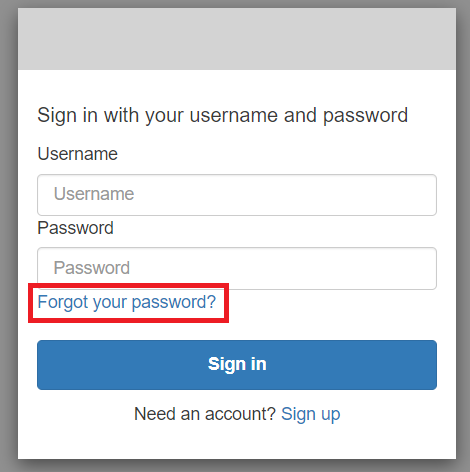
\includegraphics[width=8cm]{sezioni/images/psw-forgot.png}
        \centering
        \caption{Link per recuperare la password durante il login}
    \end{figure}

    Dopo aver cliccato, verrà inviato un codice all'email con cui era avvenuta la registrazione. Sarà neccessario infatti inserire: 
    \begin{itemize}
        \item Code;
        \item New Password;
        \item Enter New Password Again.
    \end{itemize} 
    La nuova password deve rispettare sempre le specifiche generali.
    \begin{figure}[H]
        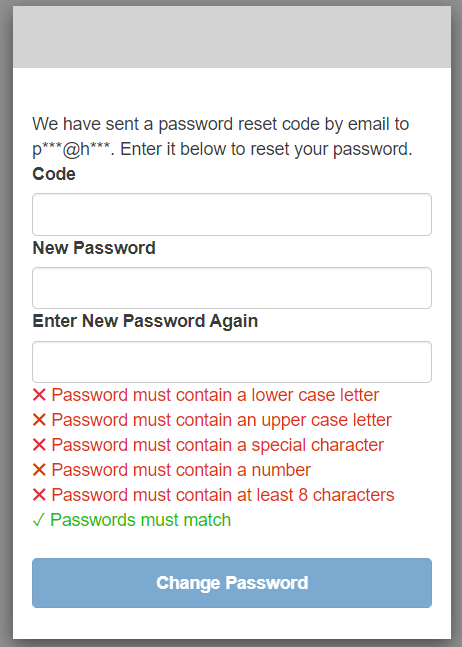
\includegraphics[width=8cm]{sezioni/images/rec-psw.png}
        \centering
        \caption{Campi da inserire durante il recupero password}
    \end{figure}

    \subsection{Credenziale nomeutente errata} {
        Se il campo del nomeutente non viene inserito, il sistema rilverà un errore di questo tipo: infatti non è possibile lasciare 
        tale campo vuoto.

        Se il nomeutente non esiste, verrà rilevato questo tipo di errore: 

        INSERIRE LE FOTO, NON CONOSCO ANCORA BENE LA PROCEDURA
    }
}

	
	\newpage
	\section{Account} {
    Dopo aver eseguito con successo la registrazione o il login, l'utente avrà accesso alla piattaforma \platform. Da questo momento
    è possibile accedere alla pagina di account, cliccando sulla barra di navigazione il bottone "\textbf{Account}". L'utente verrà reindirizzato
    in una nuova pagina contente tale informazioni: 
    \begin{itemize}
        \item Nomeutente
        \item Indirizzo email 
        \item Il numero di follower(ovvero il numero di profili social ch eti seguono)
        \item Scelta della visualizzazione della guida
        \item Modifica password
        \item Mostra seguaci
        \item Logout
    \end{itemize}

    I primi due sono esattamente i campi che si sono compilati nel modulo di registrazione.
    Mentre il pulsante logout è già stato trattato precedente. 

    \subsection{Scelta visualizzazione guida} {
        L'utente può decidere la vista predefinita che vuole per visualizzare la guida nella pagina principale. 
        Le opzioni sono 2: 
        \begin{itemize}
            \item lista: ovvero comparirà una lista di posti 
            \item mappa: i luoghi saranno posizionati all'interno di una mappa
        \end{itemize}
    }

    \subsection{Modifica password} {
        L'utente autenticato ha diritto di modificare la propria password in un qualsiasi momento. 
        ....(ora non è ancora sicuro che abbiamo ciò)
    }

    \subsection{Mostra seguaci} {
        L'utente cliccando sull'estionsione della tendina visulizzerà una lista dei profili social che segue. 
        Ognuno è associato ad uno username e dai followers (numero di persone che seguono tale profilo social). 
        Inoltre è possibile cliccare sul bottone "\textbf{Rimuovi}" per smettere di seguire un certo profilo social. 
    }

}


	\newpage
	\section{Home} {
    Quando l'utente entra nella piattaforma si trova nella pagina iniziale ``\textbf{Home}''. \aCapo
    Se non ha deciso in precedenza la visione predefinita della guida, visualizzerà i luoghi sotto forma di una mappa. 
    Direttamente dalla pagina Home, si può cambiare la visualizzazione in mappa e viceversa (da mappa in lista), cliccando tale bottone:
    \begin{figure}[H]
        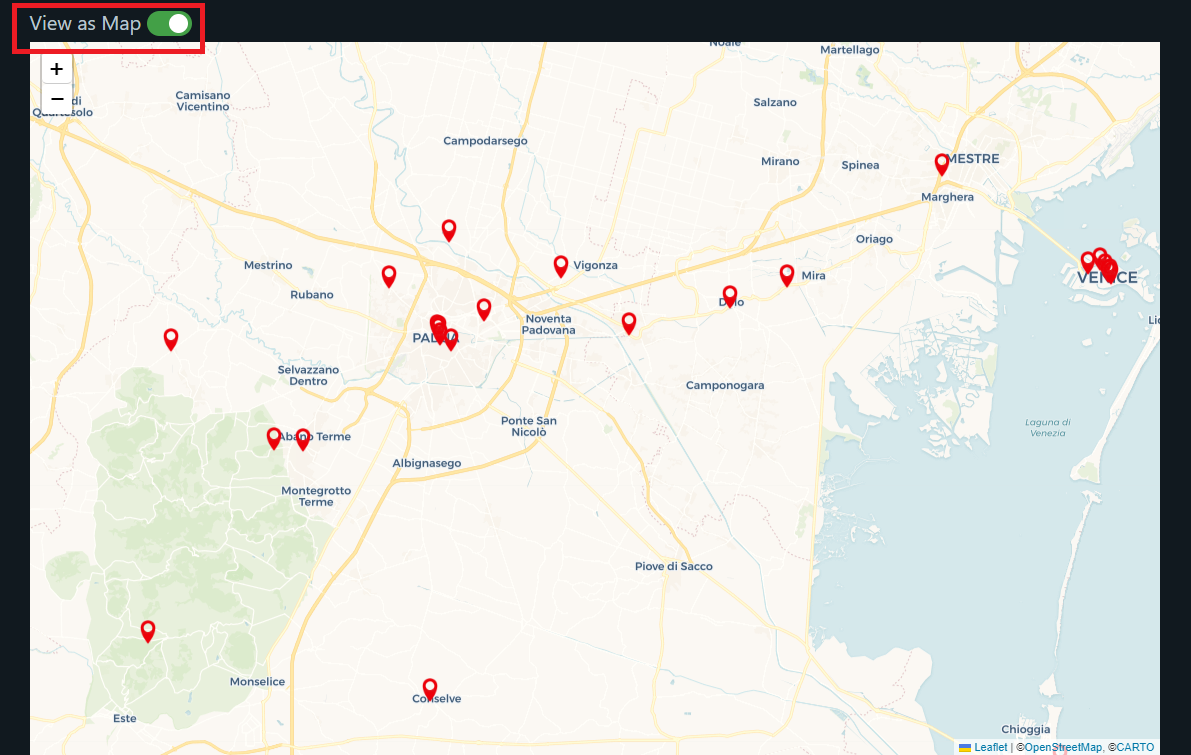
\includegraphics[width=12cm]{sezioni/images/home.png}
        \centering
        \caption{Visualizzazione predefinita della pagina Home}
    \end{figure}

    \subsection{Visualizzazione guida come lista} {
        L'utente vedrà un elenco di posti, generati dalle recensioni dei profili social seguiti dagli utenti della piattaforma \platform{}. \aCapo
        Ogni luogo è caratterizzato da tali informazioni: 
        \begin{itemize}
            \item Location: si tratta del nome del posto ed è un link, il quale una volta cliccato aprirà un popup con maggiori informazioni (§8.3); 
            \item Score: si tratta del punteggio che è attribuito al posto, su una scala da 0 a 5 stelle.
        \end{itemize}       
        \begin{figure}[H]
            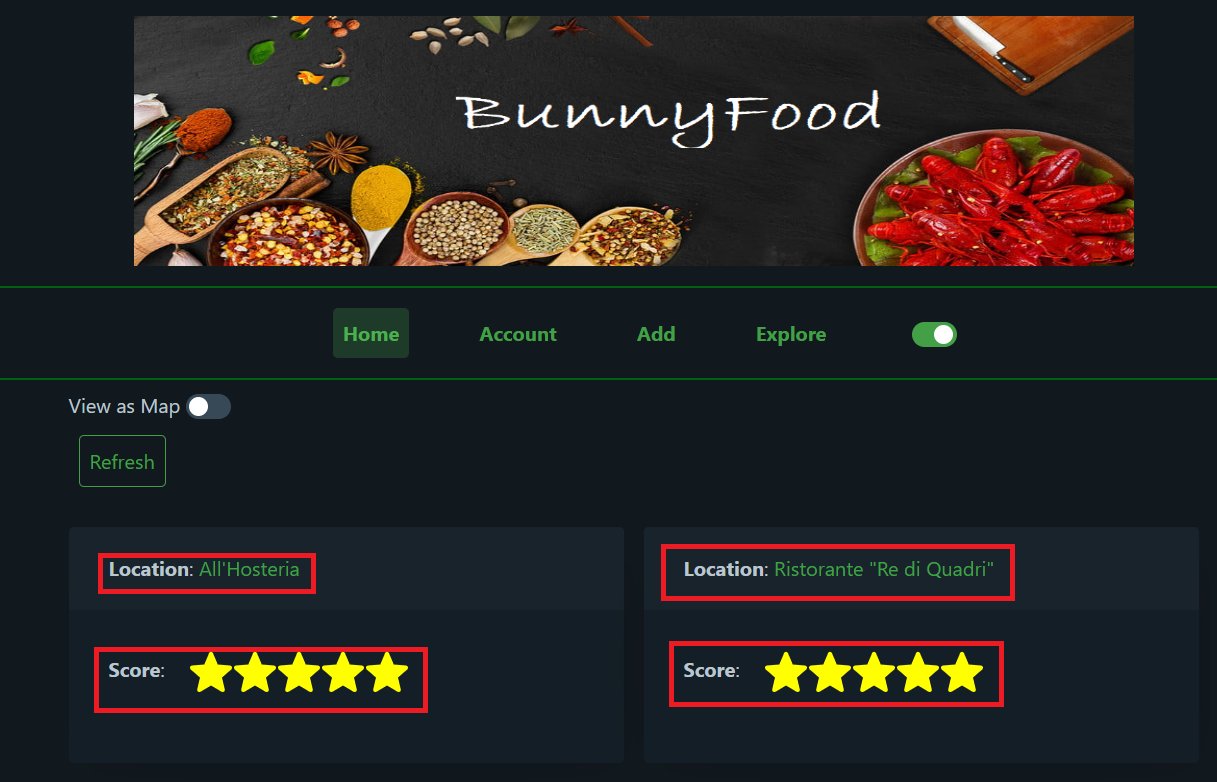
\includegraphics[width=12cm]{sezioni/images/list-home.png}
            \centering
            \caption{Visualizzazione lista locali nella pagina Home}
        \end{figure}
    }

    \subsection{Visualizzazione guida come mappa} {
        L'utente visulizzerà una mappa vera e propria con un ``segnaposto'' per la posizione di ogni posto. È possibile spostarsi sulla mappa, ingrandendo o diminuendo la visualizzazione. 
        Sono presenti infatti anche i tasti ``+'' e ``-'' per facilitare l'operazione di zoom. \aCapo
        Se il ``segnaposto'' viene cliccato compare il nome del luogo e il suo punteggio su una scala da 0 a 5. Il nome del posto, se cliccato, farà aprire un popup con maggiori informazioni (§8.3).

    }

    \subsection{Popup con maggiori informazioni} {
        Le informazioni che compaiono sono le seguenti:
        \begin{itemize}
            \item Il nome del posto;
            \item Una foto caratteristica di quel posto;
            \item Le categorie a cui appartiene il locale;
            \item L'indirizzo dove è situato il posto;
            \item Il numero telefonico del locale;
            \item Il suo punteggio su una scala da 0 a 5 stelle;
            \item Il link per il sito web di quel locale.
        \end{itemize}

        Per chiudere la finestra è necessario cliccare il tasto ``\textbf{Close}'' situato in alto a sinistra.
        \begin{figure}[H]
            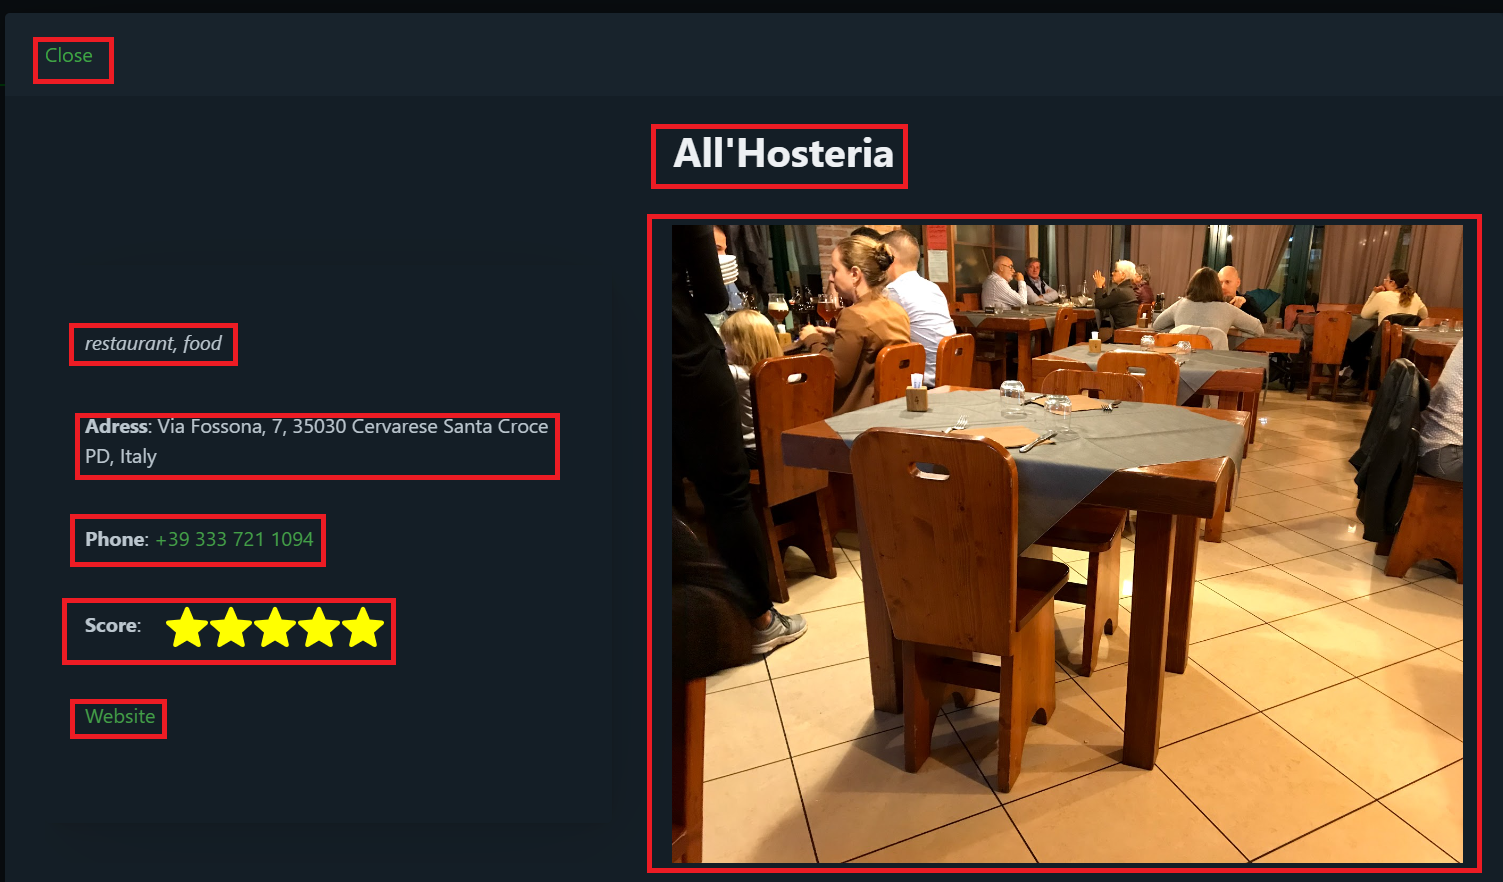
\includegraphics[width=12cm]{sezioni/images/popup.png}
            \centering
            \caption{Visualizzazione maggiori informazioni di un locale}
        \end{figure}
        }
}


	\newpage
	\section{Aggiungi un nuovo profilo} {
    Dalla pagina iniziale Home è possibile accedere alla pagina "\textbf{Add}" cliccando sulla barra di navigazione il pulsante con tale scritta.
    \aCapo
    In questa pagina, utilizzando la barra di ricerca, è possibile cercare un profilo che non si segue, scrivendo il suo nome utente e cliccando poi il bottone di "\textbf{Search}". 
    
    \begin{figure}[H]
        
\includegraphics[width=12cm]{sezioni/images/add.png}
        \centering
        \caption{Cercare un nuovo profilo social}
    \end{figure}
    
    Successivamente comparirà il profilo che si è cercato con le seguenti informazioni:
    \begin{itemize}
        \item Username del profilo;
        \item Il suo numero di followers (persone che lo seguono);
        \item Il bottone "\textbf{Segui}" che una volta cliccato permetterà di aggiungere il profilo a quelli seguiti.
    \end{itemize}

    \begin{figure}[H]
        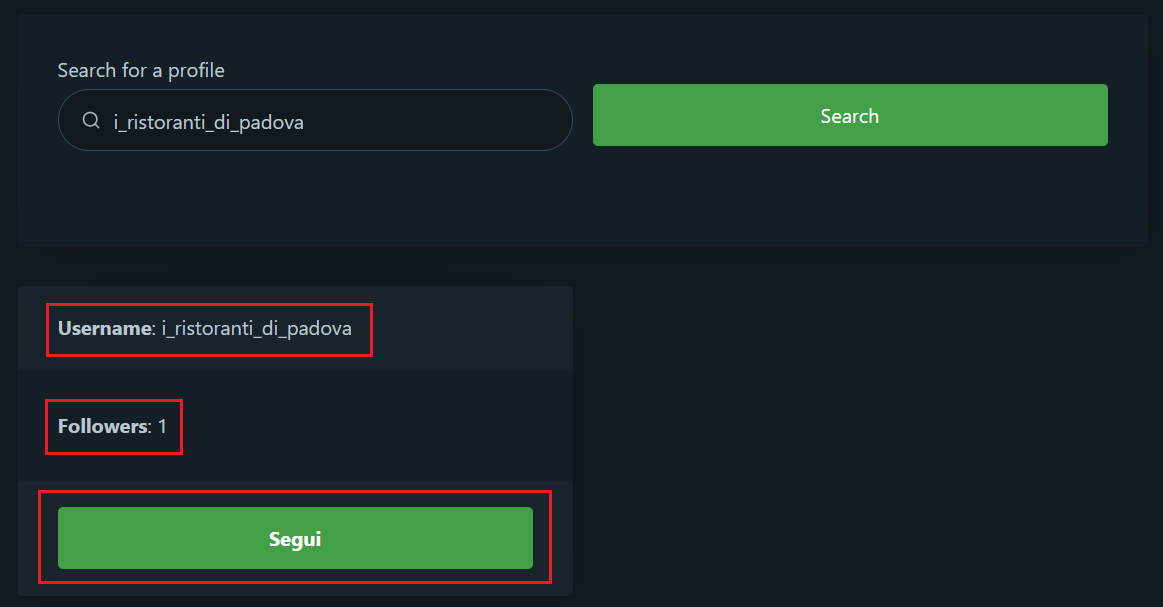
\includegraphics[width=12cm]{sezioni/images/risultato-add.png}
        \centering
        \caption{Risultato del profilo social cercato}
    \end{figure}

    \subsection{Errore nome utente} {
    \begin{enumerate}
        \item Se il campo di compilazione rimane vuoto, il sistema rileverà un errore, mostrando il seguente messaggio: 
        \begin{figure}[H]
            
\includegraphics[width=12cm]{sezioni/images/err1-add.png}
            \centering
            \caption{Errore - non è stato scritto nessun nomeutente}
        \end{figure}
        \item Se invece il nomeutente non è scritto correttamente, il sistema non riuscirà a trovare il profilo. Infatti la ricerca avviene puramente sul contenuto scritto all'interno della barra di ricerca.
        \begin{figure}[H]
            
\includegraphics[width=12cm]{sezioni/images/err2-add.png}
            \centering
            \caption{Errore - il nomeutente cercato non esiste}
        \end{figure}
        \item Se invece il nomeutente cercato è già tra i profili seguiti, comparirà un errore di questo tipo:
        \begin{figure}[H]
            
\includegraphics[width=12cm]{sezioni/images/err3-add.png}
            \centering
            \caption{Errore - il nomeutente cercato è già seguito}
        \end{figure}
    \end{enumerate}
    }
}


	\newpage
	\section{Explore} {
    Dalla pagina iniziale Home è possibile accedere alla pagina "\textbf{Explore}" cliccando sulla barra di navigazione il pulsante con tale scritta.

    La pagina contiene una lista di profili social che l'utente non segue, e gli vengono suggeriti in quanto sono i profili più virali, con maggiori followers.
    Infatti per ogni profilo social suggerito compare:
    \begin{itemize}
        \item Username: ovvero il suo nome utente;
        \item Followers: ovvero il numero di persone che seguono tale profilo social;
        \item Segui: un bottone che quando viene cliccato aggiunge il profilo social alla lista dei profili seguiti.
    \end{itemize}
}

	
\end{document}
